%chapter 4
\chapter{Josephson Junction}

\section{Josephson Junction Simulation}
\begin{figure}[h]
\centering
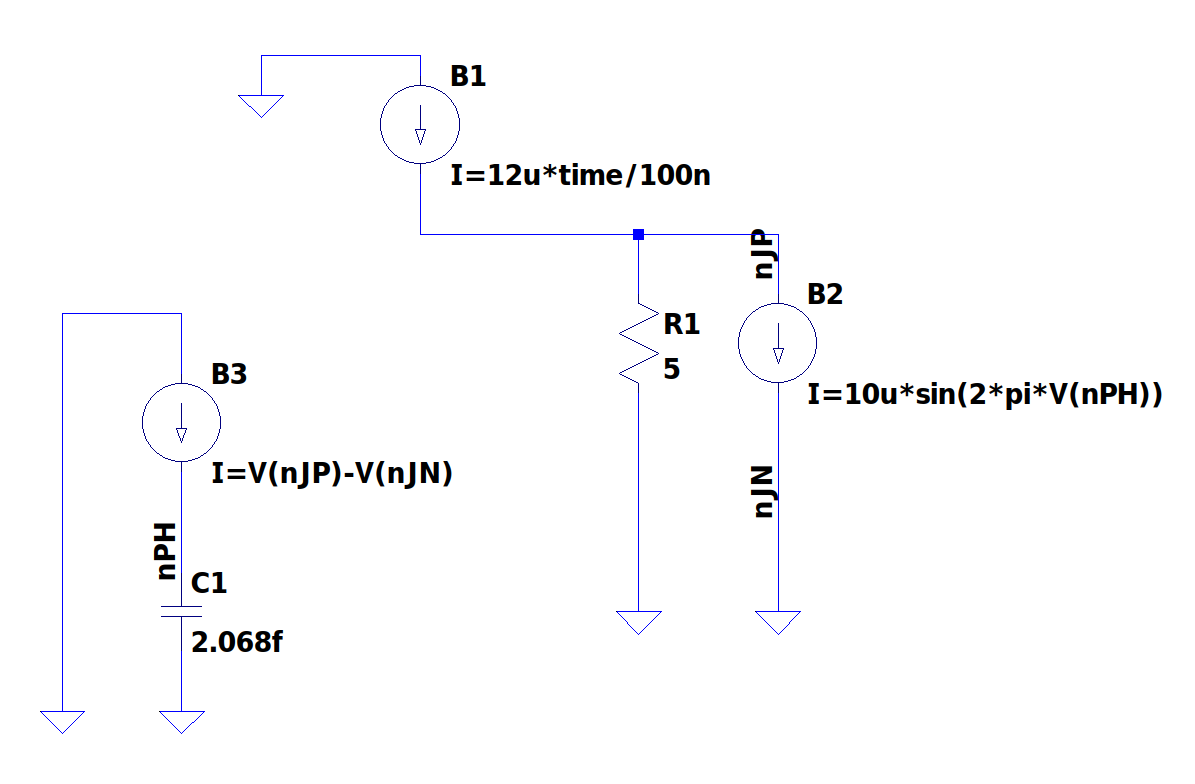
\includegraphics[width=0.7\linewidth, height=0.35\linewidth, keepaspectratio]{./exercise 4/JosephsonJunction.png}
\caption{Parallel RLC circuit implemented in LTspice}
\label{fig:ltspice}
\end{figure}

The circuit shown in Figure~\ref{fig:ltspice} models a Josephson junction using a parallel RLC configuration.
The left branch, composed of the controlled source $B3$ and the capacitor $C1$, has the role of generating the model of the phase evolution across the junction. 
The source $B2$ models the Josephson supercurrent $I_s = I_c \sin(\phi)$, while $R1$ represents the normal resistive channel of the junction. 
Finally, $B1$ provides a time-dependent bias current that drives the junction.

\section{AC Josephson Effect}
\begin{figure}[H]
\centering
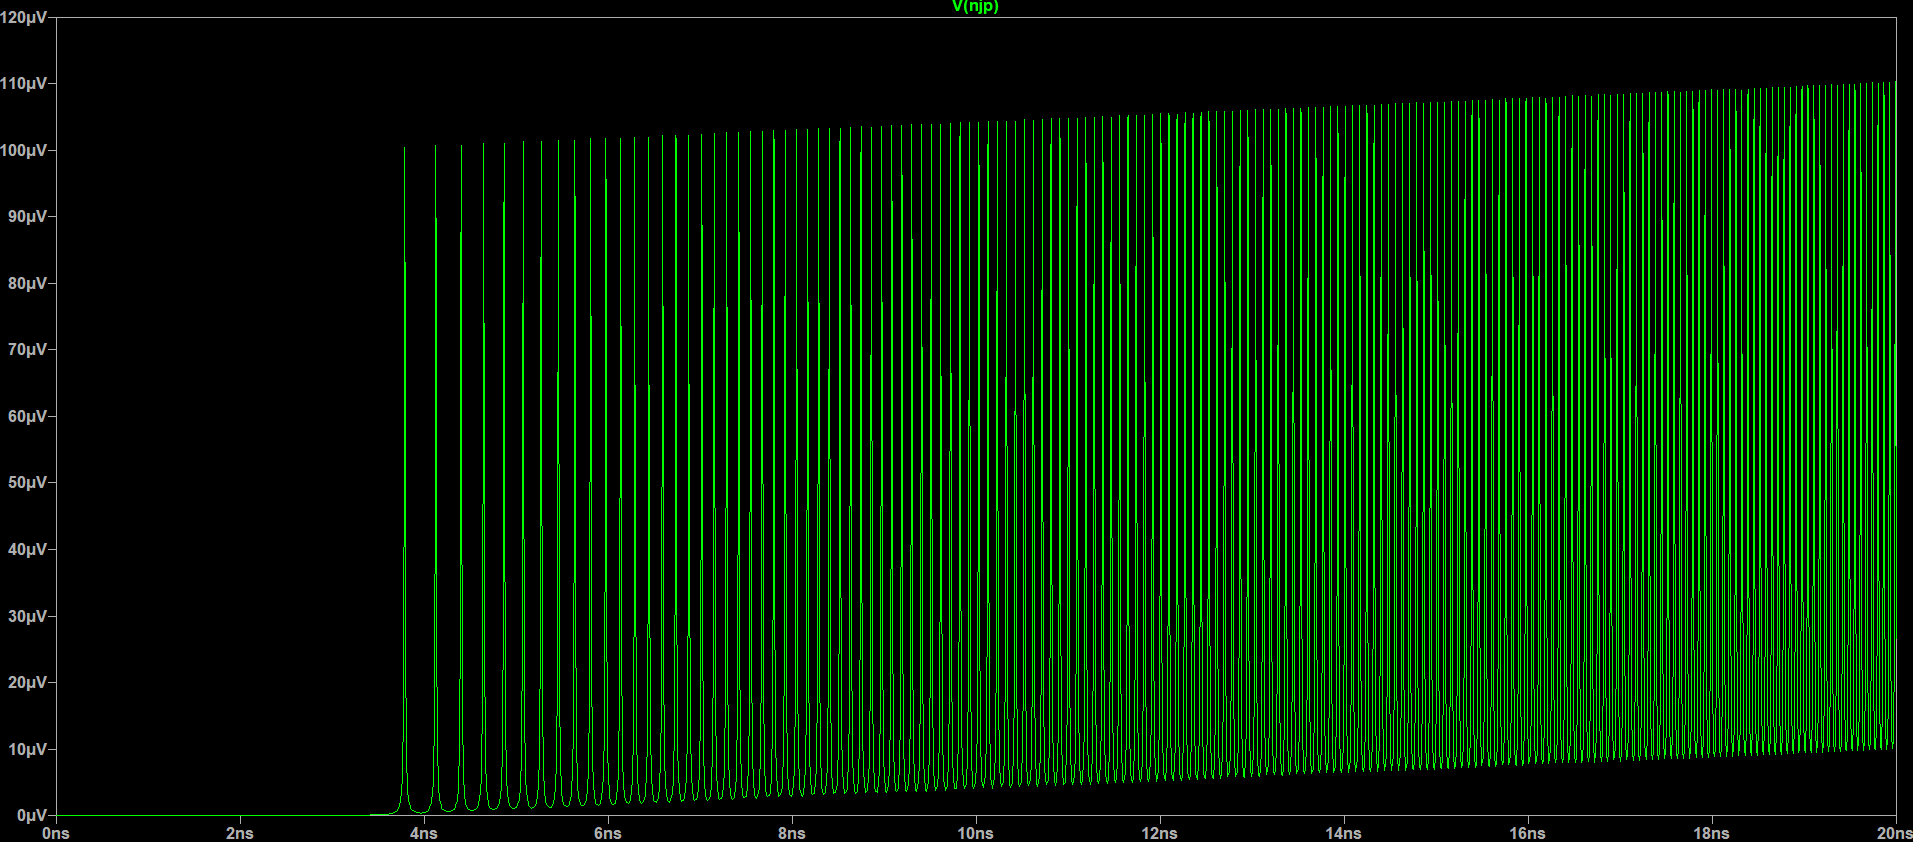
\includegraphics[width=0.8\linewidth]{./exercise 4/ACJeffect.png}
\caption{Voltage across the junction showing the AC Josephson effect.}
\label{fig:three_peaks_AC}
\end{figure}
The voltage across the junction, as shown in Figure~\ref{fig:three_peaks_AC}, exhibits a series of peaks that correspond to the AC Josephson effect.
As the bias current exceeds the critical current $I_c$, the junction transitions into a voltage state where the phase evolves in time, leading to oscillations in the voltage.
The time intervals between the peaks decrease as the bias current increases, which is consistent with the Joseph voltage–frequency relation, where the frequency of oscillation is proportional to the voltage across the junction.

\section{Time analysis of the peaks}
\begin{table}[H]
\centering

\begin{minipage}{0.45\textwidth}
\centering
\begin{tabular}{c @{\hspace*{0.5cm}} c}
\hline
Peak & Time (ns) \\
\hline
\text{peak 1} & 83.785\\
\text{peak 2} & 84.122\\
\text{peak 3} & 84.399\\
\text{peak 4} & 84.643\\
\text{peak 5} & 84.866\\
\hline
\end{tabular}
\caption{Peak times}
\end{minipage}
\hfill
\begin{minipage}{0.45\textwidth}
\centering
\begin{tabular}{c @{\hspace*{0.5cm}} c}
\hline
Interval & $\Delta t$ (ns) \\
\hline
1 $\rightarrow$ 2 & 0.337 \\
2 $\rightarrow$ 3 & 0.277 \\
3 $\rightarrow$ 4 & 0.244 \\
4 $\rightarrow$ 5 & 0.223 \\
\hline
\end{tabular}
\caption{Time differences between peaks}
\end{minipage}

\end{table}

From the peak times reported in Table~\ref{tab:peaks}, we observe that the time interval between consecutive peaks decreases slightly, meaning that the peaks become progressively closer in time. 
This behavior is expected because once the bias current exceeds the critical current ($I_c = 10\,\mu\mathrm{A}$), the junction enters the voltage state and the phase evolves according to the Josephson voltage–frequency relation 
\[
f = \frac{2e}{h}V .
\]
As the bias current increases, the mean value of voltage across the junction also increases due to the resistive branch of the model, and this can be observed in the ascending pattern of the voltage peaks. 